

\subsubsection{AES}
\\
The energy, delay and area estimates for each architecture / frequency combination is given in TABLE VII.
In Fig. 10, Fig. 11 we show the Power-Delay and Area-Delay plot for AES.

\begin{table}[h!]
\caption{Energy / Delay / Area for each architecture/frequency combination}
\begin{center}
{\begin{tabular}{c | c c c c c c c c}
\hline
AES &\multicolumn{2}{c}{1x2} &\multicolumn{2}{c}{1x0} &2x0 &2x2 &4x2 &4x0 \\ [1ex]
\hline
Frequency (MHz)& 45.45&71.42 & 45.45& 71.42& 71.42& 71.42& 71.42& 45.45 \\ [1ex]
Energy (uJ) &310.97 & 386.03 &147.38 & 144.664 &560.07 &157.58 &846.28 &177.5 \\ [1ex]

Delay (ms)& 1.21& 0.769& 0.67 & 0.43& 0.762& 0.418& 0.759& 0.655\\[1ex] 
Area (mm^2)& 7.67 & 9.03& 6.63 & 6.5 & 13& 7.5& 20.25& 9.4\\[1ex]
\hline
\end{tabular}}
\label{diffstruc}
\end{center}
\end{table}


\begin{figure}[h!]
{\centering \resizebox*{6in}{4in}{\includegraphics{aesp.ps}} \par}
\caption{Power-Delay plot for AES}
\end{figure}

\begin{figure}[h!]
{\centering \resizebox*{6in}{4in}{\includegraphics{aesa.ps}} \par}
\caption{Area-Delay plot for AES}
\end{figure}


